

%%%%%%%%%%%%%%%%%%%%%%%%%%%%%%%%%%%%%%%%%
% Journal Article
% LaTeX Template
% Version 1.4 (15/5/16)
%
% This template has been downloaded from:
% http://www.LaTeXTemplates.com
%
% Original author:
% Frits Wenneker (http://www.howtotex.com) with extensive modifications by
% Vel (vel@LaTeXTemplates.com)
%
% License:
% CC BY-NC-SA 3.0 (http://creativecommons.org/licenses/by-nc-sa/3.0/)
%
%%%%%%%%%%%%%%%%%%%%%%%%%%%%%%%%%%%%%%%%%

%----------------------------------------------------------------------------------------
%	PACKAGES AND OTHER DOCUMENT CONFIGURATIONS
%----------------------------------------------------------------------------------------

\documentclass[10pt]{article} % Single column

%\documentclass[twoside,twocolumn]{article} % Two column

\usepackage{blindtext} % Package to generate dummy text throughout this template 

\usepackage[sc]{mathpazo} % Use the Palatino font
\usepackage[T1]{fontenc} % Use 8-bit encoding that has 256 glyphs
\linespread{1.05} % Line spacing - Palatino needs more space between lines
\usepackage{microtype} % Slightly tweak font spacing for aesthetics

\usepackage[spanish]{babel} % Language hyphenation and typographical rules

\usepackage{algorithm}
	
\usepackage[hmarginratio=1:1,top=32mm,columnsep=20pt]{geometry} % Document margins
\usepackage[hang, small,labelfont=bf,up,textfont=it,up]{caption} % Custom captions under/above floats in tables or figures
\usepackage{booktabs} % Horizontal rules in tables

\usepackage{lettrine} % The lettrine is the first enlarged letter at the beginning of the text

\usepackage{enumitem} % Customized lists
\setlist[itemize]{noitemsep} % Make itemize lists more compact

\usepackage{abstract} % Allows abstract customization
\renewcommand{\abstractnamefont}{\normalfont\bfseries} % Set the "Abstract" text to bold
\renewcommand{\abstracttextfont}{\normalfont\small\itshape} % Set the abstract itself to small italic text

\usepackage{titlesec} % Allows customization of titles
\renewcommand\thesection{\Roman{section}} % Roman numerals for the sections
\renewcommand\thesubsection{\roman{subsection}} % roman numerals for subsections
\titleformat{\section}[block]{\large\scshape\centering}{\thesection.}{1em}{} % Change the look of the section titles
\titleformat{\subsection}[block]{\large}{\thesubsection.}{1em}{} % Change the look of the section titles

\usepackage{fancyhdr} % Headers and footers
\pagestyle{fancy} % All pages have headers and footers
\fancyhead{} % Blank out the default header
\fancyfoot{} % Blank out the default footer
\fancyhead[C]{Dise\~no y An\'alisis de Algoritmos. \textbf{Proyecto \# 3: Kevin el encargado}} % Custom header text
\fancyfoot[RO,LE]{\thepage} % Custom footer text

\usepackage{titling} % Customizing the title section

\usepackage{hyperref} % For hyperlinks in the PDF

\usepackage{graphicx} % For images

\usepackage{pifont} % bullets

\usepackage{amsmath}

\usepackage{algpseudocode}

% Keywords command
\providecommand{\keywords}[1]
{
	\small	
	\vspace{0.5em}
	\noindent \textbf{\textit{Palabras clave --- }} #1
}


%----------------------------------------------------------------------------------------
%	TITLE SECTION
%----------------------------------------------------------------------------------------

\setlength{\droptitle}{-4\baselineskip} % Move the title up

\pretitle{\begin{center}\Huge\bfseries} % Article title formatting
	\posttitle{\end{center}} % Article title closing formatting
\title{\normalsize{Dise\~no y An\'alisis de Algoritmos }\\
	\Huge\bfseries Proyecto \# 3: Kevin el encargado \\
} % Article title
\author{% 
	
\includegraphics[height=6cm]{logo.png} \vspace{1em}\\
	Laura Victoria Riera P\'erez\\
	Mari\'e del Valle Reyes \vspace{1em} \\
	\small Cuarto a\~no. Ciencias de la Computaci\'on. \\ % institution
	\small Facultad de Matem\'atica y Computaci\'on, Universidad de La Habana, Cuba \\ % institution
}
\date{\footnotesize \today } % Leave empty to omit a date


% Abstract configurations
\renewenvironment{abstract}
{\small
	\begin{center}
		\bfseries \abstractname\vspace{-.5em}\vspace{0pt}
	\end{center}
	\list{}{
		\setlength{\leftmargin}{1.5cm}%
		\setlength{\rightmargin}{\leftmargin}%
	}%
	\item\relax}
{\endlist}

\usepackage{amsthm}
\usepackage{amssymb}
\usepackage{todonotes} % \TODO
\usepackage{listings} % Code listings
\usepackage{xcolor}

\definecolor{backcolour}{rgb}{0.95,0.95,0.92}

\newcommand{\csl}[1]{\colorbox{backcolour}{\texttt{#1}}}

\newcommand{\imgcaption}[2]{\tiny \textbf{Figura #1.} #2.}

\newcommand{\mgc}[2][]{\colorbox{backcolour}{\texttt{\_\_#2\_\_#1}}}

\newcommand{\mgccapt}[1]{\texttt{\_\_#1\_\_}}

\newtheorem{thm}{Teorema}
\newtheorem{mydef}{Definici\'on}%[section]
\newtheorem{lem}{Lema}
\newtheorem{fig}{\scriptsize{Figura}}
\newtheorem{col}{Corolario}


\renewcommand{\qedsymbol}{\rule{0.7em}{0.7em}}

% Hyperlinks configurations
\hypersetup{
	colorlinks=true,
	linkcolor=black,
	filecolor=magenta,      
	urlcolor=cyan,
	pdftitle={Overleaf Example},
	pdfpagemode=FullScreen,
}

%----------------------------------------------------------------------------------------

\begin{document}
	% Print the title
	\maketitle
	
	%----------------------------------------------------------------------------------------
	%	ARTICLE CONTENTS
	%----------------------------------------------------------------------------------------
	
	\section{Repositorio del proyecto}
	
	\begin{center}
		\href{https://github.com/computer-science-crows/algorithms-design-and-analysis}{https://github.com/computer-science-crows/algorithms-design-and-analysis}
	\end{center}

	\section{Definici\'on inicial del problema} 

	Kevin ha sido puesto al frente de la comisión de la facultad que elegirá las fechas de las pruebas de los k cursos que se dan en la facultad.
	
	Cada curso tiene una cantidad de pruebas determinadas que quiere poner, y propone para esto, por ejemplo, los días \{ 17, 34, 65 y 87 \} del curso escolar, si vemos a este como una sucesión de días en los que se imparten clases. Para mostrarse flexibles, los cursos a veces elaboran más de una propuesta incluso.
	
	Por un problema de desorganización las propuestas se regaron y ahora no se sabe que curso propuso que propuesta, pero ya Kevin esta cansado de tanta gestión. Kevin quiere elegir k propuestas que ninguna quiera poner pruebas el mismo día que las otras, así supone que todo el mundo estará contento, ayude a Kevin.
	

	\section{Definici\'on en t\'erminos matem\'atico - computacionales}\label{section_2}
	
	La entrada de nuestro problema es el n\'umero \textit{k} de cursos impartidos en el semestre y una lista \textit{p} que contiene al menos \textit{k} propuestas. Una propuesta es una lista con d\'ias del curso escolar en donde podr\'ian efectuarse las pruebas de un curso. El objetivo es encontrar una cantidad \textit{k} de propuestas sin d\'ias en com\'un para formar el calendario de ex\'amenes. La salida del problema es una lista con una combinaci\'on posible de propuestas en caso de existir, de lo contrario, se ofrecen disculpas a Kevin y se retorna una lista vac\'ia.
	
%	\subsection{Problema de Selecci\'on de Actividades}
%	El problema de selección de actividades es un problema de optimización clásico que se ocupa de la selección de la cantidad m\'axima de actividades no concurrentes que se pueden realizar en un marco de tiempo determinado. 
	
	\subsection{Teor\'ia de grafos}
	Este problema tambi\'en puede ser resuelto utilizando el enfoque de la teoría de grafos, model\'andolo como un grafo donde cada nodo representa una propuesta, y una arista entre dos nodos indica que las propuestas correspondientes tienen alg\'un d\'ia en com\'un. 
	
	\begin{mydef}
		Sea $G = (V, E)$ un grafo. $A \subseteq V$ es un conjunto independiente de $G$ si el subgrafo inducido por $A$ no tiene aristas.  
	\end{mydef}
	
	Un conjunto independiente en este caso, constituir\'ia un conjunto de propuestas que no tienen di\'as en com\'un. El problema estar\'ia en buscar un conjunto independiente de tama\~no \textit{k}.
	
	\section{Problema NP: M\'aximo conjunto independiente}
	
	\section{Soluciones implementadas}
	
	\subsection{Backtrack}
	
		Como primera solución al problema fue implementado un \textit{backtrack}. Esta es una solución correcta, ya que  genera todas las combinaciones posibles de k propuestas y verifica si cumplen con la restricción de que no haya dos cursos con exámenes el mismo día. La complejidad temporal de este algoritmo es $O(n^k)$, donde n es el número de propuestas. En una computadora de 32GB de RAM, intel core i7-11na generación, se puede resolver para una cantidad máxima \todo{ajustar al problema actual}. Dicha solución puede ser encontrada en src/solutions/backtrack\_solution.py.
		
	\subsection{Programaci\'on lineal}
	
	Este problema puede ser modelado tambi\'en como un problema de optimizaci\'on lineal. Sea $ x_{i} $ una variable binaria que indica que se tom\'o el v\'ertice $ i $. Se quiere maximizar la suma de $ x_i \forall i \in V $. Las restricciones a\~nadidas  garantizan que ning\'un par de v\'ertices elegidos sean vecinos, y por tanto la soluci\'on hallada sea un conjunto independiente. 
		
	\begin{equation} \left\{
		\begin{matrix}
			\max & \displaystyle z=\sum_{i \in V}x_{i}\\
			\textrm{s.a.} & x_i + x_j \leq 1 & \forall (i, j) \in E \\
			& x_i \in \{0, 1\} & \forall i \in V \\ 
		\end{matrix} \right. 
	\end{equation} 
	
	Esta soluci\'on fue implementada utilizando la librer\'ia \textit{PuLP} y puede ser encontrada en \textit{src/solutions/linear\_prog\_solution.py}. La complejidad temporal para resolver problemas con PuLP depende del solucionador subyacente que se utilice. Por defecto, PuLP usa COIN-OR Branch and Cut Solver (CBC), el cual se basa en el método simplex y es combinado con otros algoritmos. La complejidad temporal del método simplex es generalmente $O(n^2 \cdot log(n))$ (el caso peor es $O(2^{n} $), pero en general es bastante r\'apido), donde \textit{n} es el número de variables en el problema. Sin embargo, debido a los algoritmos adicionales utilizados por CBC, la complejidad temporal real puede variar según la instancia específica del problema.
	
	%La complejidad temporal del simplex para el caso peor es O($ 2^{n} $), pero en general es bastante r\'apido.
	
	\subsection{Metaheur\'istica: Algoritmo gen\'etico}
	
	En la resoluci\'on del problema se utiliza el algortimo gen\'etico como metaheur\'istica. La implementación se basa en representar las soluciones como una lista binaria del mismo tamaño que la lista de propuestas de entrada. En esta representación, un valor de 1 en un índice indica que esa propuesta ha sido seleccionada, mientras que un valor de 0 indica que no ha sido seleccionada.
	
	El objetivo del algoritmo genético es encontrar una lista binaria con exactamente k valores de 1, lo que representa la selección de k propuestas sin que ninguna de ellas tenga días comunes. Para lograr esto, se emplean dos operadores principales: mutación y cruzamiento.
	
	La operación de mutación consiste en intercambiar posiciones en la lista binaria. Esto permite explorar nuevas soluciones al cambiar las propuestas seleccionadas. Por ejemplo, si se encuentra un 1 en un índice, se puede intercambiar ese valor con otro índice donde haya un 0 y viceversa.
	
	El operador de cruzamiento, o crossover, se aplica a dos listas binarias. Dado un índice i, se intercambian todos los elementos hasta el índice i de una lista con los elementos de la otra lista. Esto permite combinar características de ambas soluciones y explorar nuevas posibilidades.
	
	La función de evaluación se encarga de determinar la calidad de una solución. En este caso, devuelve un número positivo si la lista binaria es válida, es decir, si cumple con las restricciones de que las propuestas seleccionadas no tengan días comunes. Por el contrario, devuelve un número negativo si la lista binaria no es válida.
	
	El algoritmo genético continúa iterando hasta encontrar una lista binaria válida que cumpla con las restricciones. Se generan nuevas soluciones aplicando mutación y crossover, y se seleccionan las mejores soluciones para la siguiente generación, utilizando la función de evaluación como criterio de selección.
	
	\subsection{Aproximaciones}
	
	Los algoritmos de aproximación son una técnica poderosa para tratar problemas de optimización NP-hard, proporcionando garantías comprobables sobre la distancia de la solución devuelta a la óptima. Estos algoritmos son particularmente útiles cuando una solución exacta es intratable y se puede encontrar rápidamente una solución casi óptima.
	
	\subsubsection{Greedy}
	
	\subsubsection{Random}
	
	\subsubsection{Bellman-Ford}
	
	\section{Generador de casos de prueba}
	
	En \textit{src/app/generator.py} fue implementado un generador, el cual recibe una cantidad $ s $ de muestras a producir, genera valores random con el formato de entrada de los algoritmos implementados, halla la soluci\'on \'optima con $ backtrack $ y las guarda en $ json/test\_cases.json $. Se generaron 3000 casos de prueba.
	
	\section{Tester}
	En \textit{src/app/tester.py} fue implementado un tester, que recibe una funci\'on y prueba el desempe\~no de la misma en cuanto a si obtuvo la soluci\'on \'optima o no, y el tiempo que demor\'o en hacerlo, comparando con los casos de prueba obtenidos con el generador. Adem\'as, estos resultados se guardan en un $ .json $ con el nombre de la funci\'on en la carpeta tests. La soluci\'on implementada fue testeada para todos los casos de prueba generados y puede encontrarse en $ json/tests/corruption\_strategy\_solution.json $ .
	
	\section{Comparaci\'on de soluciones implementadas}          

%    A continuaci\'on se muestra una gr\'afica por cada algoritmo con el tiempo que demor\'o en cada uno de los 3000 tests. Como podemos observar, en los casos analizados, el \textit{backtrack} puede demorar desde 0.000 hasta 0.016 segundos en ejecutarse, pero la mayor\'ia de los casos oscilan entre 0.000 y 0.002. La \textit{soluci\'on con flujo} para todos los casos se demora menos de 0.0016 segundos, lo cual lo convierte en una soluci\'on significativamente mejor que el backtrack.
%    
%    \begin{center}
%    	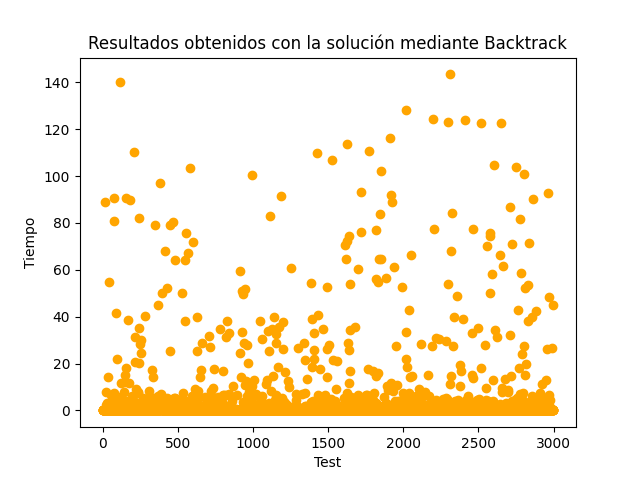
\includegraphics[width=7cm]{Backtrack_results.png}
%    	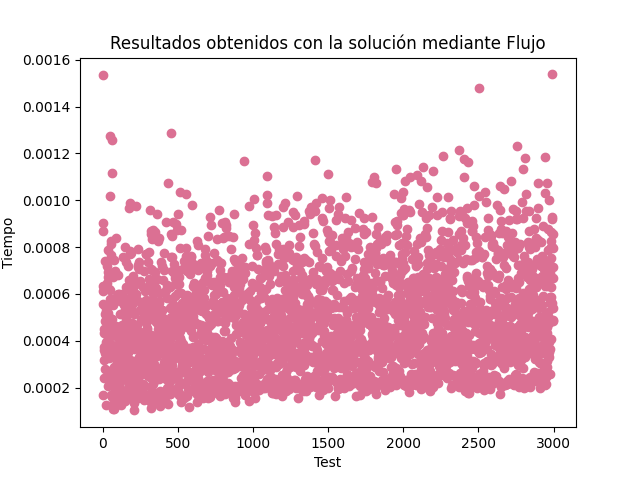
\includegraphics[width=7cm]{Flujo_results.png}
%    \end{center}  
%    
%    Adem\'as, en la siguiente gr\'afica se ofrece una comparaci\'on del tiempo promedio que le toma a cada algoritmo ejecutar los casos de prueba. 
%    
%    \begin{center}
%    	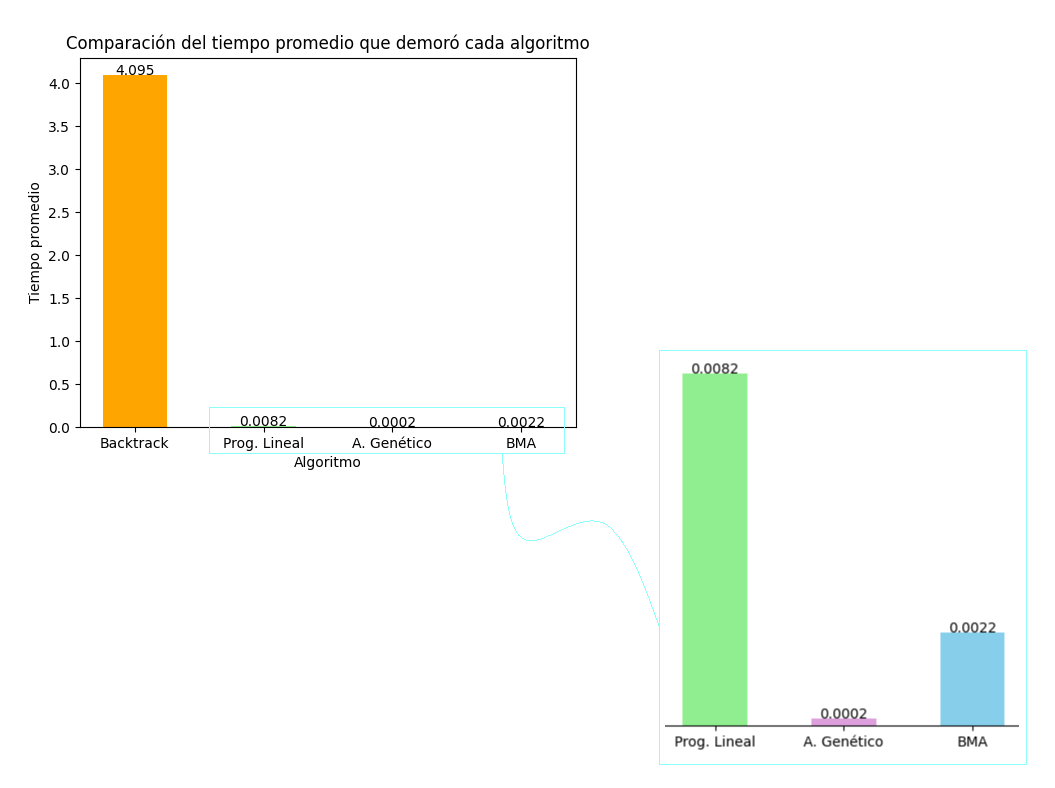
\includegraphics[width=7cm]{Bar_comparative_plot.png}
%    \end{center}
%	
%	\begin{center}
%		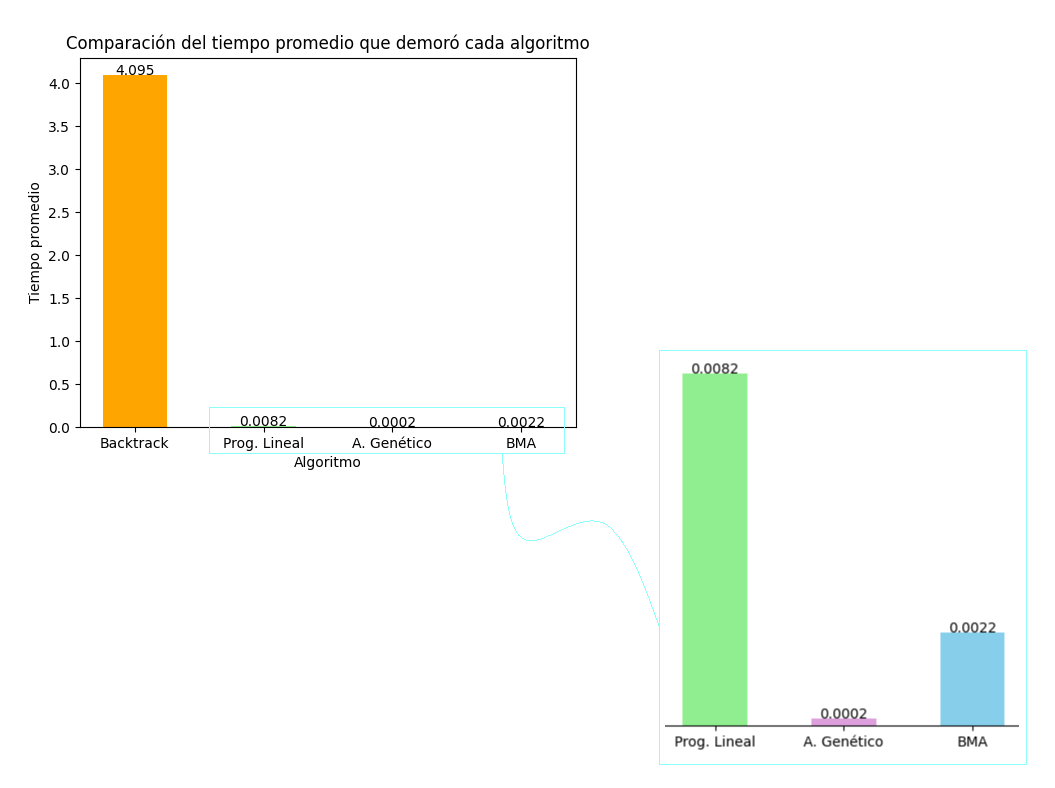
\includegraphics[width=7cm]{Bar_comparative_plot.png}
%	\end{center}
	
	\begin{thebibliography}
		a
		\bibitem{introduction} Cormen, Thomas H. y otros. \emph{Introduction to Algorithms}. 
		The MIT Press.
		4ta Edici\'on.		
		Cambridge, Massachusetts.
		2022.
	\end{thebibliography}
\end{document}


